
\subsection{\ref{exp:design:4} - gRPC Maximum Throughput}
\label{sec:experiments:results:per-experiment:04}
% Goal: To evaluate how meshed configurations behave with alternative communication protocols.

In the final experiment we utilize a different type of application workload. In the previous experiments we evaluated the different configurations and \gls{sm} systems using various HTTP workloads. In this experiment, we use a different application level protocol to evaluate how the layer-7 aware data plane proxies perform with alternative layer-7 application protocols. 



\begin{figure}
\centering
\makebox[\linewidth][c]{
    \begin{minipage}{.6\textwidth}
      \centering
      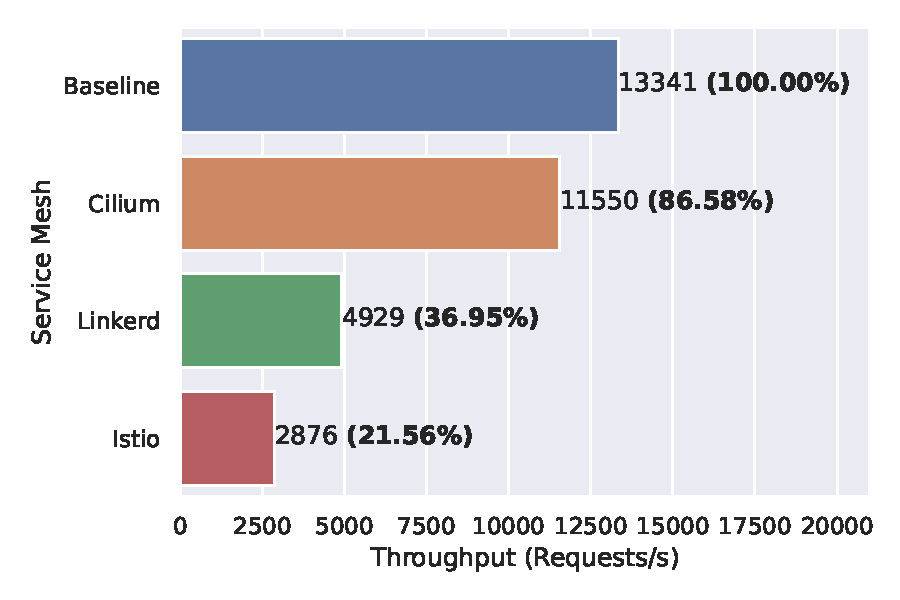
\includegraphics[width=\linewidth]{5_experimental_evaluation/figures/exp-04-max-throughput.pdf}
      \caption[Average throughput of \gls{sm} systems under maximum load using the gRPC protocol]{Average throughput of \gls{sm} systems under maximum load using the gRPC protocol.\\}
      \label{fig:exp:04:maximum-throughput}
    \end{minipage}
    
    
    \begin{minipage}{.6\textwidth}
      \centering
      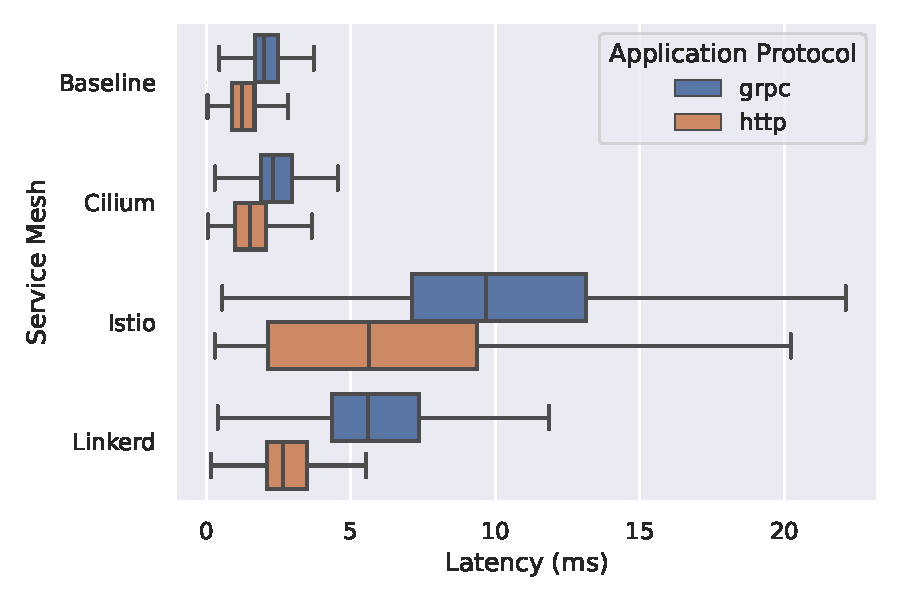
\includegraphics[width=\linewidth]{5_experimental_evaluation/figures/exp-04-latency-compared.pdf} 
      \caption[Comparing the latency distributions of \gls{sm} systems under maximum load for both HTTP and gRPC workloads]{Comparing the latency distributions of \gls{sm} systems under maximum load for both HTTP and gRPC workloads.}
      \label{fig:exp:04:latencies-compared}
    \end{minipage}
}
\end{figure}


\subsubsection{Maximum Sustained Throughput Analysis}
\label{sec:experiments:results:per-experiment:04:throughput}

In \cref{fig:exp:04:maximum-throughput} we present a bar chart which depicts the average throughput a \gls{sm} system was able to process throughout the 15-minute duration of the experiment. During this experiment, the workload generator produced as many requests as the receiving system was able to process and did so in an unrestricted manner. The results are presented in the chart which can be interpreted as follows. On the y-axis we present the different \gls{sm} configurations. The x-axis presents the aggregated average throughput value that a configuration was able to process, expressed in requests per second. The values next to the bars represent the actual observed value and the percentage next to it represents the percentage of throughput a system was able to process compared to the best performing configuration, which in this case is the baseline.


The very first thing to notice in \cref{fig:exp:04:maximum-throughput} is the absence of Traefik in the depicted chart. This is because the proxy in Traefik was unable to process any gRPC requests and any attempt in doing so resulted in errors even though historical articles produced by the vendor explicitly state the support for the gRPC protocol \cite{maesh-introduction}. This leads to our tenth main finding:

\begin{shaded*}
    \noindent
    \ref{exp:mf10}:
    The configuration using Traefik was unable to process any gRPC based requests.
\end{shaded*}

% Comparison of HTTP vs gRPC (reduction of throughput)
% Cilium $16.83\%$ $13.42\%$
% Linkerd $54.94\%$ $63.05\%$ 
% Istio $80.09\%$ $78.44\%$
% Traefik $97.39\%$  - 

Another observation we can make is regarding the levels of throughput a \gls{sm} system can process compared to the baseline configuration. Similarly to the first experiment, in which we evaluated the maximum sustained throughput whilst using HTTP-based requests and responses (\cref{sec:experiments:results:per-experiment:01}), we observe that there is a significant reduction of throughput for each of the evaluated \gls{sm} systems. The best performing \gls{sm} system is once again, Cilium, experiencing a $13.42\%$ reduction in throughput compared to the baseline configuration. Linkerd is the second best performing system, which experiences a $63.05\%$ reduction. The greatest reduction of throughput, however, is reserved for the Istio which experiences a massive $78.44\%$ reduction in throughput compared to the baseline.

When we compare these results to the results from the first experiment we can observe a similar trend. We observe the same ranking whilst evaluating this metric. Additionally, the relative differences when comparing the reductions per protocol are minimal. Most of the evaluated systems experience similar reductions for both application level protocols. The largest difference observed is for Linkerd, which encountered a $54.94\%$ reduction for the HTTP workloads whilst it encountered a $63.05\%$ reduction for the gRPC based workloads. This brings us to our eleventh main finding:

\begin{shaded*}
    \noindent
    \ref{exp:mf11}:
    Both gRPC and HTTP-based workloads experience similar reductions in terms of sustained throughput.
\end{shaded*}

\subsubsection{Latency Analysis}
\label{sec:experiments:results:per-experiment:01:latency}


In \cref{fig:exp:04:latencies-compared} we present the latency distributions of the evaluated configurations under maximum load for both the gRPC and HTTP-based workload experiments. On the y-axis we present the evaluated configurations, excluding Traefik. On the x-axis we present the latency in milliseconds. The colours of the bar indicate the type of workload used. The blue bars (gRPC) present the data from the fourth experiment, whereas the orange bars (HTTP) present the observed latency values from the first experiment.


\begin{figure}[!t]
\centering
\makebox[\linewidth][c]{
    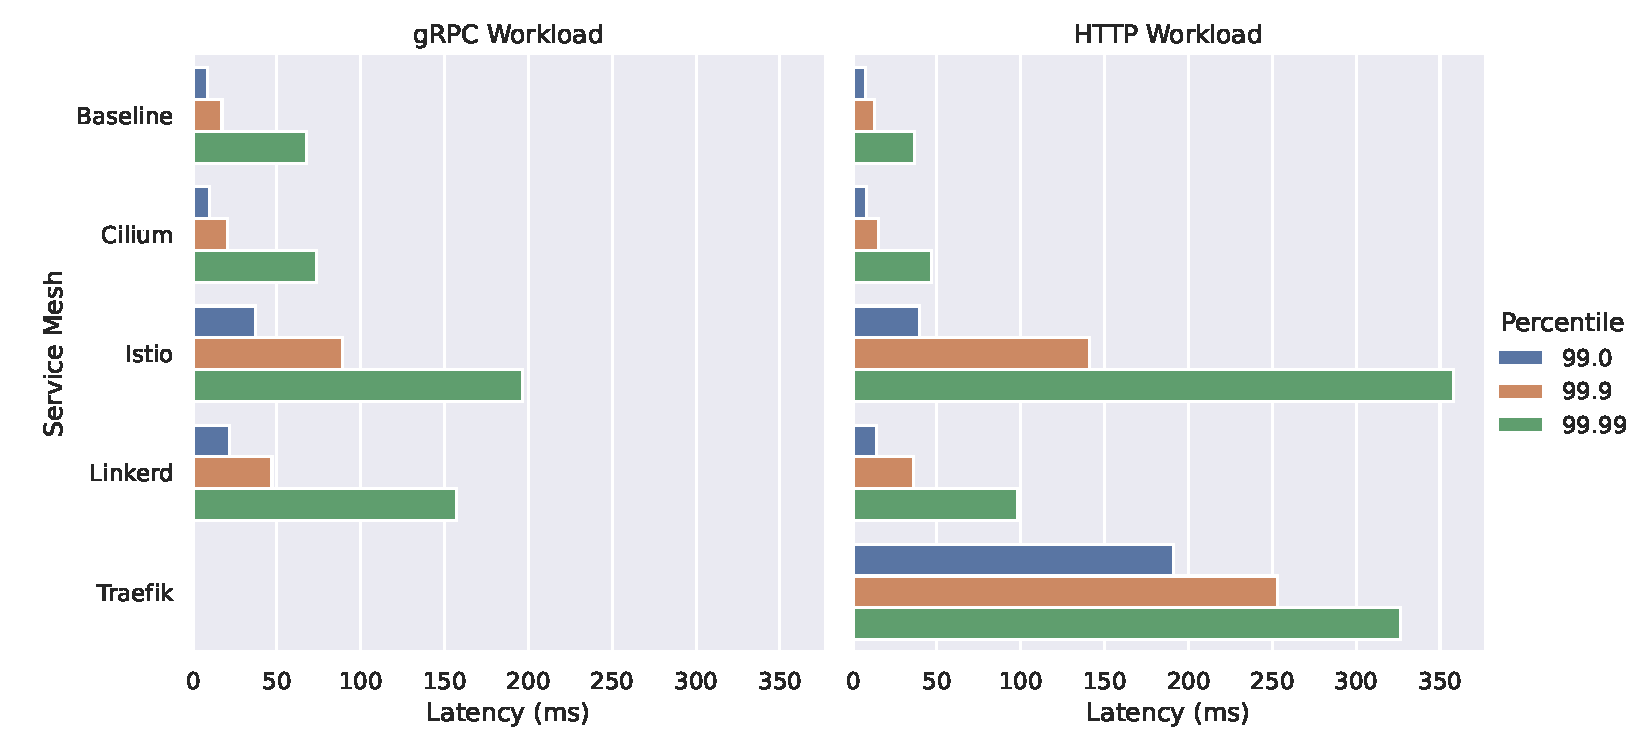
\includegraphics[width=1.2\linewidth]{5_experimental_evaluation/figures/exp-04-tail-latencies-all-compared.pdf} 
}

   \caption[Tail end latencies of \gls{sm} systems experiencing maximum load per application protocol]{Tail end latencies of \gls{sm} systems experiencing maximum load per application protocol.}
    
   \label{fig:exp:04:tail-latencies}

\end{figure}

The first observation that we can make is that the observed latency values are slightly higher for the gRPC based workloads across all the evaluated configurations. Furthermore, we can observe that the spread of latency values for Linkerd is larger when using a gRPC-based workload, compared to the HTTP-based counterpart. Although there are some differences, we can conclude that there are no significant differences in the latency distributions based on the application protocol.


In \cref{fig:exp:04:tail-latencies} take a closer look at the observed tail end latencies for both types of application level protocols used. On the y-axis we present the evaluated \gls{sm} configurations and on the x-axis we present the latency in milliseconds. Within the plots we depict coloured bars, in which the colours represent the 99th, 99,9th, and 99.99th percentile respectively. The plot on the left displays the results for the gRPC-based workload whereas the plot on the right presents the result for the HTTP-based workload.

From the plots as depicted in \cref{fig:exp:04:tail-latencies} we can observe a couple of interesting findings. First, we observe that the tail end latencies, specifically the 99.99th percentile are negatively affected whilst using the gRPC based protocol for the baseline configuration and the configurations using Cilium and Linkerd. Interestingly however, is that the tail end latencies of Istio improved significantly when exposed to gRPC-based workloads compared to the HTTP counterpart. This could be related to the manner in which the data plane proxy, Envoy, processes gRPC based requests as they treat is as a first class citizen at both the transport and application layer\footnote{\url{https://www.envoyproxy.io/docs/envoy/latest/intro/arch_overview/other_protocols/grpc}}.

